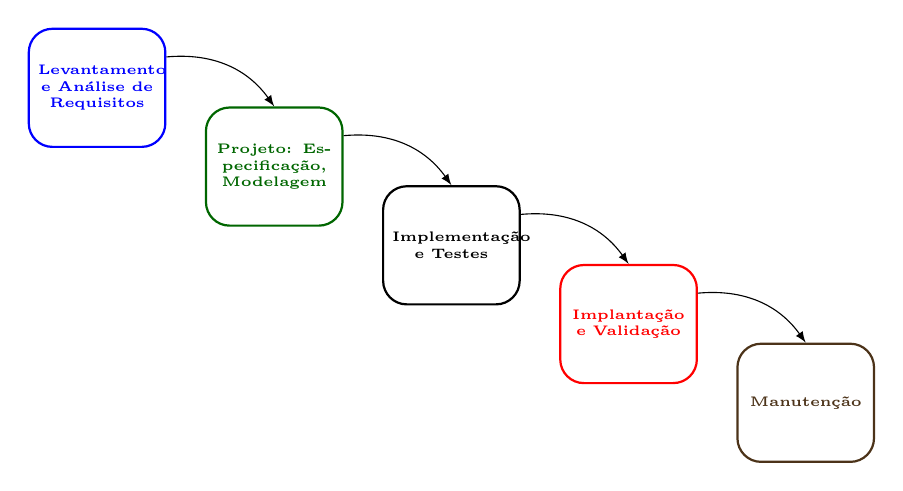
\begin{tikzpicture}
  [font={\tiny\bf},node distance=2.25cm,every path/.style={->,>=latex,draw},
  cycle/.style={thick,rounded corners=3mm,text centered,text width=1.5cm,minimum width=1cm, minimum
    height=1.5cm,draw},
  dev/.style={cycle},
  deploy/.style={cycle,red},
  maintain/.style={cycle,brown!40!black}]

  \node<1->[cycle,blue] (requirements) {Levantamento e Análise de Requisitos};
  \node<2->[cycle,green!40!black] (proj) [right of=requirements,yshift=-1cm] {Projeto: Especificação, Modelagem};
  \node<3->[dev] (dev) [right of=proj,yshift=-1cm] {Implementação e Testes};
  \node<4->[deploy] (deploy) [right of=dev,yshift=-1cm] {Implantação e Validação};
  \node<5->[maintain] (maintain) [right of=deploy,yshift=-1cm] {Manutenção};
  
  \path<2-> (requirements) edge [bend left] (proj.north);
  \path<3-> (proj) edge [bend left]  (dev.north);
  \path<4-> (dev) edge [bend left]  (deploy.north);
  \path<5-> (deploy) edge [bend left]  (maintain.north);
\end{tikzpicture}
